\documentclass[conference]{IEEEtran}
\IEEEoverridecommandlockouts
% The preceding line is only needed to identify funding in the first footnote. If that is unneeded, please comment it out.
\usepackage{cite}
\usepackage{amsmath,amssymb,amsfonts}
\usepackage{algorithmic}
\usepackage{algorithm}
\usepackage{graphicx}
\usepackage{textcomp}
\usepackage{xcolor}
\usepackage{array}
\usepackage{soul}
\def\BibTeX{{\rm B\kern-.05em{\sc i\kern-.025em b}\kern-.08em
    T\kern-.1667em\lower.7ex\hbox{E}\kern-.125emX}}
\begin{document}

\title{{A Secure Algorithm for Deep Learning Training Under GAN Attacks}\\
\author{\IEEEauthorblockN{Aseem Prashar, and Sergio A. Salinas Monroy }
\IEEEauthorblockA{\textit{Department of Electrical Engineering and Computer Science} \\
\textit{Wichita State University}\\
Wichita, USA \\
prasharaseem@gmail.com, sergio.salinasmonroy@wichita.edu }
%\and
%\IEEEauthorblockN{Sergio A. Salinas Monroy}
%\IEEEauthorblockA{\textit{Department of Electrical Engineering and Computer Science} \\
%\textit{Wichita State University}\\
%Wichita, USA \\
%sergio.salinasmonroy@wichita.edu}
}
}
\maketitle

\begin{abstract} 

Deep neural networks have outperformed traditional machine learning approaches for many tasks, and are the tool of choice in many
fields. However, directly applying these techniques in fields that deal with private data is
challenging. The reason is that a third-party, which organizations may not trust, usually needs to centrally collect private data. 
To overcome this challenge, researches have proposed distributed training algorithms that allow multiple users to collaboratively train
their local deep learning models without sharing private datasets. 
However, these approaches are vulnerable to recently proposed attacks where a malicious user can replicate private data from
another user  by compromising the collaborative training algorithm. 
In this paper, we propose a privacy-preserving distributed deep learning algorithm that allows a user to leverage the private
datasets from a group of users while protecting its privacy. Our algorithm prohibits this user from ever sharing the parameters of its
model, and thus it prevents malicious users from compromising the training and replicating the user's private data.  We conduct
extensive experiments and observe that our algorithm can achieve a  model accuracy of 95.18\%, which is the same
accuracy that previous approaches that are vulnerable to attacks can achieve. 
\end{abstract}

\begin{IEEEkeywords}
Neural Network, Deep learning, GANs
\end{IEEEkeywords}

%---------------------------------------------------------------------------------
\section{Introduction}
%---------------------------------------------------------------------------------
In the past few decades, deep learning has generated a lot of interest in the research and academic community due to its great ability
to automatically classify large amounts of data. This has led to breakthroughs in many fields ranging
from autonomous driving, and natural language processing to genetic research and speech processing 
\cite{sun2014deep,young2018recent, al2017deep, danaee2017deep,hinton2012deep}.
%It is no surprise that deep learning has seen a significant investment by technology giants such as Google, IBM and Facebook. 
This revolutionary technology is especially fruitful for large corporations that need to automatically process very large data sets to
provide deep learning inference services to their users. For example, data collection at Facebook enabled them to create DeepText, a
text understanding engine that is able to extract meaningful context from text \cite{abdulkader2016introducing}.

Although it is possible to collect large-scale data to train deep learning models in some application domains, e.g., online social
networks, there are other fields where such centralized data collection is currently infeasible due to privacy
concerns. In particular, users' data can contain instances of private information that needs to be kept secret from companies that 
centrally collect data to provide deep learning services \cite{chicurel2000databasing}. Such private data includes
%It is only inevitable that a
%subset of the sample space contains sensitive information that was accidentally captured without user consent.  Other privacy concerns
%regarding data ownership have also been raised since the trained model is generally a 
intellectual property (IP), 
%. Other %red flags are centered around 
medical data protected by Health Insurance and Portability and Accountability Act (HIPA), and student records protected by the Family
Educational Rights and Privacy Act (FERPA) \cite{act1996health,blechner2002health,shultz2015your}. 
%While medical
% community
%By sharing their data, organization can receive improved deep learning inference. However, 
%stands to benefit from deep learning, 
%the privacy concerns around these type of data make it impossible to share with an untrusted third-party such as a deep learning
%service provider. 
%medical history of patients makes collecting of data samples a challenging task. 

Instead of sharing private data with a third-party, users could locally train their own deep learning models using their own
data. However, since a single user only has access to a relatively small data set, its locally 
trained deep learning model has low accuracy. Moreover, locally trained models can suffer from over generalization that can prevent
them from being used in practical scenarios. Hence, it is necessary to develop secure training algorithms that can achieve
high accuracy while preserving privacy.  . 

% For instance, a hospital trained a deep neural network to
%recognize patients with pneumonia based on their
% chest X-ray images using its own records. Although this neural network was successful in classifying records from patients that were
% treated in this hospital, its performance significantly dropped when tested with images from patients treated at a different
% hospital \cite{zech2018variable}. This was due to the fact that the trained deep neural network learned to identify particular imaging
% machine used at the hospital instead of the content of the image itself. 
%This indicates that models trained on single source datasets
% can produce confounding results.
%Moreover, many organizations may not have large enough local data sets to train a deep learning model with satisfactory
%accuracy. 
%Accessibility of training datasets in hospital that do not have sufficient resources or samples currently is also a concern.
 
Researchers have proposed several techniques to enable privacy-preserving training of deep learning neural networks. Specifically,  
researchers have used secure multiparty computations (SMC) to encrypt users' private data and distribute the training computations over
many users, which preserves users' privacy 
\cite{ ma2018privacy,sheikh2010distributed,miyajima2016new,bonawitz2017practical}. 
This approach, however, is impractical for most users since the encryption computations in SMC add a significant computational
overhead and they are required to be online during the training.   

Differential privacy has also been proposed to protect users' data privacy in deep learning training
\cite{vepakomma2018no,abadi2016deep,chase2017private}. By adding artificial noise to the training data,
differential privacy allows a remote server to train a deep learning model without learning individual data
samples. However, the accuracy of the deep learning model under a large number of users decreases due
to the additional noise needed to protect their privacy. Thus, differential privacy suffers from poor scalability. 

More recently,  Shokri et al.  \cite{shokri2015privacy} researchers have proposed privacy-preserving distributed learning. In this
approach, users locally train a deep neural network using their own data sets. Users then upload a small subset of their model
parameters to a server, where they  are aggregated. The server then sends the aggregated parameters back to the users, who can use
them to improve their local models. Since users only share their model parameters with the server, they avoid directly disclosing their
private data sets to the server of other users. Under this algorithm, the deep learning models at the users can achieve a high
accuracy. 

Unfortunately,  the approach \cite{shokri2015privacy} is vulnerable to the generative adversarial network (GAN) attack described by 
Hitaj  et al. \cite{hitaj2017deep}, where  a malicious user is able to replicate data samples from a victim user. In this attack, 
the malicious user uploads specially crafted model parameters to the aggregation server, which are eventually downloaded by the victim
user to train its local model. The victim trains its local model using the compromised aggregated parameters, which results in
update model parameters that contain private information about its data samples. Since the victim uploads its compromised model
parameters to the server, the malicious user gains access to them. By iteratively feeding the aggregate parameters that contain private
information about the victim's data sample to its GAN, the malicious user can replicate the victim's data samples, and thus compromise its
privacy.

In this paper, we propose a novel privacy-preserving distributed deep learning framework that prevents the GAN attack described in 
\cite{hitaj2017deep} while allowing the users to train their local models with high accuracy. 
Specifically, instead of attempting to protect the privacy of all users as in \cite{shokri2015privacy}, we focus on protecting the
privacy of a single user, called the reference user. The GAN attack in \cite{hitaj2017deep} exploits 1) the uploaded
model parameters from the victim, and 2) the fact that the  aggregation server unconditionally accepts model parameters from any user
in the system, which could potentially be malicious. Therefore, in our algorithm, we prohibit the reference user from uploading its
model's parameters to the server, and the server only accepts parameters from randomly selected users at each iteration. 
To verify the efficacy of our approach, we run extensive experimental evaluations on Amazon Web Service's Elastic
Compute Cloud (AWS EC2). We observe that our approach maintains the accuracy of the deep learning model compared to a training
algorithm that does not protect privacy, even when the number of users who are allowed to upload parameters to the aggregation
server is reduced. We also measure the trade-off between privacy and accuracy, and show that the main user can easily choose the most
appropriate trade-off by tuning the user selection probability. 

%our proposed algorithm works as follows. First, all users train a local deep learning model using only their local data.
%Second, the algorithm randomly selects a set of users to upload their parameters to be aggregated by the server. The reference user is
%prohibited form uploading its model parameters. Third, the reference user and the selected users update their local deep
% learning models with the newest aggregated parameters. The iteration continues until the reference user's deep learning model
% achieves
%a minimum accuracy, or a maximum number of iterations is reached.

% The main contribution of our approach is that it allows the main user to leverage the data sets form the other users to train a local
% deep learning model with high accuracy while protecting its private data from the parameter server, and other users who
% may launch sophisticated GAN based attacks as described in \cite{hitaj2017deep}. The proposed architecture is independent of the
% neural network architecture of the system, and is therefore, adaptable to any deep neural network. Our proposed privacy-preserving
% distributed learning approach can potentially be used in a scenario where the privacy of one of the participant in distributed learning is valued over other participants. For instance, a medical facility that has classified medical data can still benefit from distributed deep learning using our approach. 

%---------------------------------------------------------------------------------
\section{Problem Formulation}
%---------------------------------------------------------------------------------
In this section, we first provide a brief background on deep learning, and then describe our considered system and threat models. 


%---------------------------------------------------------------------------------
\subsection{Deep Neural Networks}
%---------------------------------------------------------------------------------
Before delving into details about our system model, we describe the architecture of deep neural networks and their training methods. 
%------------------------------------------------------------------------------
\subsubsection{Architecture}\label{sec:MLP}
%------------------------------------------------------------------------------
\begin{figure}[t]
\centering
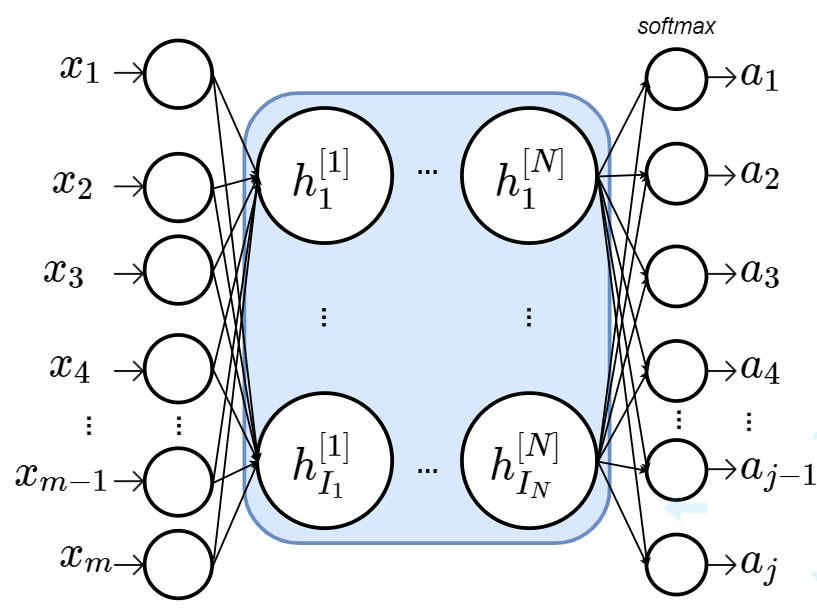
\includegraphics[width=0.3\textwidth, keepaspectratio]{SimpleNN}
\caption{A neural network with $m$ inputs, $j$ outputs,  $N$  hidden layers, and $I$ neurons per layer.}
\label{fig:SimplNN}
\end{figure}
In this work, we use the multilayer perception (MLP), one of the most common deep neural network architectures. 
%An MLP is formed by input, hidden, and output layers where each layer consists of many nodes. Each node takes
%as input a weighted average of the previous layer's node outputs, and the output of an special node called the bias.  
%The nodes use a non-linear activation function to compute their output. Together, the weights and
%biases are called the parameters of the deep neural network. %We show a typical MLP architecture in Fig. \ref{fig:SimplNN}. 
Figure \ref{fig:SimplNN} shows the structure of a typical classification MLP with $m$ input nodes, $j$ outputs nodes, and  
$N$ hidden layers. Each layer has $I$ neurons. Intuitively, this MLP takes a data sample represented as a vector of length
$m$ on its input layer, and outputs the probability that it belongs to the $j$th category on the $j$th output neuron.

The output of the $i$th neuron at layer $k$ is defined as is given by 
$$a_k=f(W_k a_{k-1}),$$
where $f$ is the activation function, $W_k$ is the weight matrix of layer $k$,
and $a_{k-1}$ is the vector of neuron outputs from the the $k-1$th layer. 
We denote the flattened vector of all weights of the MLP by $w$. 
%There are several non-linear activation functions that can be used for function $f$, including sigmoid,
%hyperbolic tangent, and rectified linear unite (ReLU) \cite{Goodfellow-et-al-2016}. In this
%work, we will focus on the ReLU activation function:
%$$f(z) = \max\{0, z\},$$
%where given an input $z$ the function returns $z$ for positive values and $0$ for negative values.

% The output layer is usually implemented with the SoftMax activation function. The output of this function is between zero and
% one, and it is used to the output of the last hidden layer to a scalar that represents the probability that the data sample observed at
% the input layer belongs to each of the $j$ categories. Formally, the SoftMax activation functions is defined by
% $$f(z)_j = \frac{e^{z_j}} {(\sum_ke^{z_k})} \ \  \forall j,$$
% where $z_j$ is the $j$th element of the input vector $z$ with $k$ elements (e.g., the output of all the neurons in the last hidden
% layer).

We note that our results and formulations are generalizable to other deep neural network architecture besides the MLP. 

%---------------------------------------------------------------------
\subsubsection{Training}\label{sec:training}
%---------------------------------------------------------------------
Before a neural network can be used to perform inference, e.g., classify images, it needs to be trained to learn the highly non-linear
relationships between the inputs and the correct outputs. 

To train the MLP in Section \ref{sec:MLP}, we use the stochastic gradient descent (SGD) algorithm, which aims to find the 
the weights $W_k$ for all layers $k$ that result in the inferences with the highest accuracy.  SGD is an iterative algorithm where each
iteration has two steps: forward propagation and back propagation.

In the forward propagation step, the SGD algorithm feeds a randomly
selected subset of samples, called the mini-batch, one by one to the MLP, and collects the MLP's output for each sample based on the
current value of its weights.
Then, the SGD computes the error function, which measures the difference between the outputs of the neural network and the correct 
classification solutions, which we call labels. In this work, we use the mean squared error function, i.e., 
\begin{align}\label{eq:errorFunction}
 E= \frac{1}{n} \sum_{n=1}^{n}(y_i -\hat{y_i}),
\end{align}
where $n$ is the the number of samples in the training dataset, $y_i$ is the output calculated by the neural network and 
$\hat{y_i}$ is the correct label for the $i$th sample.

Next, in the back propagation step, the SGD algorithm 
computes the partial derivative of the error function with respect to the
parameters of each neuron in the deep neural network, which indicate how much each parameter contributed to
the error. Based on the partial derivatives, the SGD algorithm updates the MLP's parameters.
 Specifically, the $j$th parameter of the flattened vector of parameters $w$ is given by:
\begin{align}\label{eq:SGD}
w_j = w_j -\alpha \frac{\partial E_i}{\partial w_j}, 
\end{align}
where $E_i$ is the value of the error function defined in \ref{eq:errorFunction} computed over
minibatch $i$, $\alpha$ is the learning rate, and  $\frac{\partial E_i}{\partial w_j}$ denotes the partial derivative of $E_i$ with
respect to parameter $w_j$.

The SGD algorithm continues with the forward pass, error calculation, back propagation and parameter update iteration until a minimum
error is achieved or a maximum number of iterations is reached \cite{ruder2016overview}. 


%---------------------------------------------------------------------------------
\subsection{System Model} \label{sec:systemModel}
%---------------------------------------------------------------------------------
\begin{figure}[t]
\centering
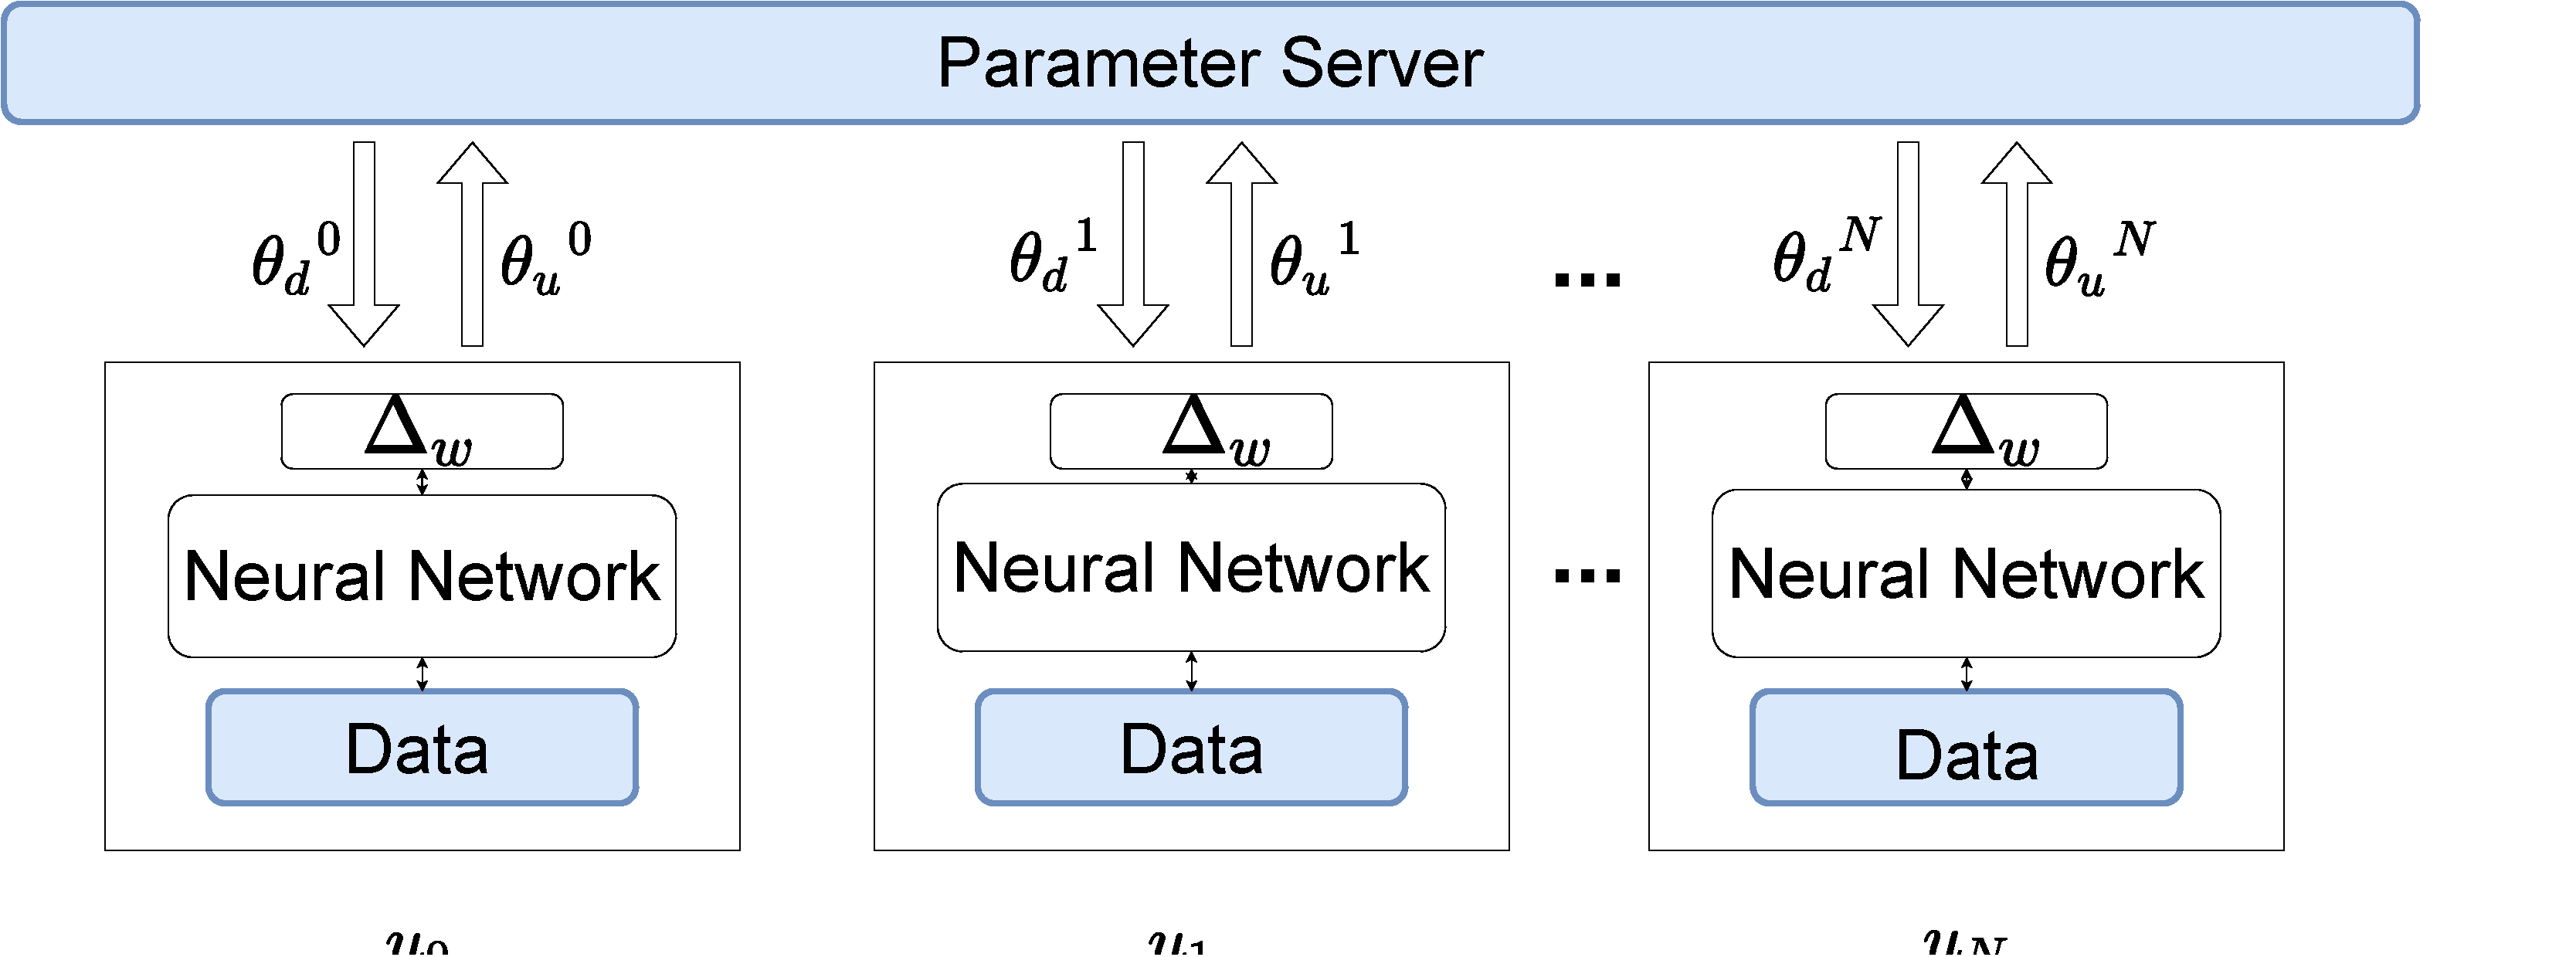
\includegraphics[width=0.4\textwidth, keepaspectratio]{HighLevelArch.pdf}
\caption{An architecture for privacy-preserving distributed learning.}
\label{fig:HighLevel}
\end{figure}
 
We consider a distributed deep learning system formed by a set of $N$ users $\mathcal{U}= \{u_0, \dots,u_N\}$ and
a parameter server (PS). User $u_0$ aims to train a local deep neural network using its own training data set
$d_{u_0}$ as well as the data sets of the other users $d_{u_i}$. 
The training data sets $d_{u_i}$'s of all users contain private information that cannot be shared with each other or with the PS.  We
assume the training data set at the reference user is significantly smaller  than the total training data available in the system.
Otherwise, the reference user could achieve a comparable accuracy without having to participate in the distributed learning. 
User $u_0$'s deep neural network is a multilayer perceptron (MLP) as described in Section \ref{sec:MLP} for image classification.


% Table \ref{table:1} summarizes the notations used in this work.
% \begin{table}[!h]
% \centering
% \caption{Table1: Summary of notations used in the paper}
% \label{table:1}
% \begin{tabular}{ | m{0.12\columnwidth} | m{0.8\columnwidth}| } 
% \hline
% \textbf{Notation} & \textbf{Description} \\
%  \hline\hline
% 
% $N$ & Number of participants except the system\\
% \hline
% $u_0$ & Reference User and the  main benefactor of the architecture \\
% \hline
% $M$ & Mini batch size used for stochastic gradient descent\\
% \hline
% $\theta_u^{i}$ & Fraction of parameters selected for upload from total available parameters for $i$th user \\
% \hline
% $\theta_d^{i}$ & Fraction of parameters selected for download from total available parameters for $i$th user\\
% \hline
% $W_k$ & Weight matrix for layer K in the neural network\\
% \hline
% $w_i$ & Flattened vector of all parameters in the neural network. \\
% \hline
% $\Delta w_i$ & Vector of changes in all local parameters due to SGD\\
% \hline
% $w^{(global)}$ & Flattened parameter vector for server\\
% \hline
% $E$ & Error function defining the difference between the computed value and expected value of the objective function \\
% \hline
% $E_i$ & Error function defining...\\% the difference between the computed value and expected value of the objective function \\
% \hline
% $\alpha$ & Learning rate of the stochastic gradient descent algorithm\\
% \hline
% $\mathcal{S}_i$ & Set of $\theta_u^{i}$ largest indices selected from $w_i$ \\
% \hline
% \end{tabular}
% \end{table}

%-------------------------------------------------------------------------
\subsection{Privacy-preserving Distributed Learning under the Semi-honest Users Threat Model}
%-------------------------------------------------------------------------
To allow user $u_0$ to train its deep learning network while preserving its privacy, we could use the distributed
learning approach proposed by Shokri et al. \cite{shokri2015privacy}. 
%This approach allows user $u_0$, as well as the rest of the users,  to use the private data from each other to train a deep learning
% model. 
In the approach proposed in \cite{shokri2015privacy}, each user $u_i\in\mathcal{U}$ trains a local deep learning
network, and uploads certain parameters of its model to a server. The server aggregates the parameters from all users and
then allows the users to download some of them. This iteration can be repeated until the accuracy of the users' local deep learning models
achieves a minimum value.
By only sharing certain parameters of their local models
with a parameter server, users avoid having to transmit any of their private samples to each other or to the server.  
%We assume that the architecture and training parameters of the deep neural network at user $u_0$ are known 
%to all other users and to the parameter server.


Specifically, let  $w^{(global)}$ and $w_i$ be the parameters at the parameter server and at user $u_i$, respectively. Let 
$\theta_d^{i}$ and $\theta_u^{i}$ be the percentage of parameters that user $u_i$ downloads and uploads, respectively. Then, 
to initialize the system,  each user $u_i$ randomly sets its parameters $w_i$ to a randomly chosen value and selects a learning rate,
$\alpha_i$. Then, at each iteration,  user $u_i$  downloads $\theta_d^{i} \times |w_i|$ parameters from the parameter server and
overwrites the corresponding parameters in $w_i$, where $|w_i|$ denotes the total number of parameters in $w_i$. User $u_i$ then runs
the stochastic gradient descent algorithm described in \ref{sec:training} with the updated parameter vector as the initial vector. 
Based on the results of the SGD,  user $u_i$ uses \eqref{eq:SGD} to calculate $w_i^{(new)}$.

Next, user $u_i$ determines which parameters to upload to the server based on how much each parameter changed compared to the previous iteration.  To
this end the user first computes
\begin{align}\label{eq:deltaParam}
\Delta w_i =  w_i^{(new)} -  w_i
\end{align}
which measures the changes between the old and new
local parameters. Then, the user forms set $\mathcal{S}_i$ with the indices of the elements in vector $\Delta w_i$ that have the top 
$\theta_u^{i} \times |\Delta w_i|$ values, where $|\Delta w_i|$ is the size of $\Delta w_i$. 
The user $u_i$ forms vector $w_{\mathcal{S}_i}$, which contains the parameters in $w_i^{(new)}$ whose indexes are in
set $\mathcal{S}_i$, and uploads it to the parameter server. Note that $w_{\mathcal{S}_i}$  is set to zero in the remaining
positions. 

After receiving the parameters from user $u_i$, the parameter server updates its own vector as follows:
$$w^{(global)} =  w^{(global)} +  w_{\mathcal{S}_i}$$
Intuitively, by using $w_{\mathcal{S}_i}$, which contains information about the parameters in the local model of $u_i$i that have
undergone the largest changes during the local SGD training, the parameter server can improve its own parameters that are then
downloaded by other users to further improve their own models.  

Although this approach can train local models with high classification accuracy,  it assumes a semi-honest threat model for the users,
which is not realistic. That is, it assumes that the users will attempt to find private information about other users based on 
the parameters that they download from the server, but do not deviate from the procedure described above. As we will see in the next
section, users can launch active attacks where they maliciously modify the parameters that they upload to recreate samples from other
users. 

%---------------------------------------------------------------------------------
\subsection{A Malicious Threat Model for Distributed Deep Learning}\label{sec:threatModel}
%---------------------------------------------------------------------------------

In this work, we consider a malicious threat model for both the parameter server and the users. Specifically, in addition to
attempting to learn private information about other users' dataset based on the parameters at the server as in the semi-honest threat
model, the attacker in the malicious threat model uploads
specially crafted parameters. The malicious parameters lead other users to upload their parameters in such a way that they disclose private information about their data sets. This information can the be downloaded and used by the
attackers to recreate private data samples from the victims. 

Such an attack has been described by Hitaj et al. \cite{hitaj2017deep}. In particular, the attack operates as follows. 
Suppose user $u_A\in\mathcal{U}$ is malicious and targets another user $u_V\in\mathcal{U}$. Further assume that all users, including
the malicious one, agree on the hyper parameters of a neural network architecture such as the number, size and type of layers,  and the
classification labels as described in Section \ref{sec:systemModel}.

The victim user $u_V$ declares that its private training data set contains samples for the  labels $[a,b]$. The adversary
$u_A$ declares to have the classification labels $[b,c]$ in its training data set, which means it declares that it has no data for
label $a$. By deploying the attack, the adversary aims to replicate samples with the same probability distributions as the private
samples with label $a$ at user $u_V$.

The adversary user $u_A$ then locally uses a generative adversarial network to generate samples that have the same distribution as
samples with label $a$ at $u_V$. The adversary labels these malicious samples as belonging to category $c$, and uses them to retrain
its local model. After the parameters from the malicious users are uploaded and aggregated by the server, the victim user $u_V$
downloads them to retrain its model. Since the compromised parameters where obtained using samples of label $a$ misclassified as label
$c$, the parameters of the retrained model that are related to identifying label $a$ will experience the largest changes, and thus
will be uploaded by the victim to the server. The adversary $u_A$ can then download the aggregated parameters that contain the
parameters from the victim user. By iteratively following this procedure, the adversary $u_A$ collects enough information about samples
of label $a$ at $u_V$ to recreate their probability distribution. 

% We summarize the attack proposed by \cite{hitaj2017deep} as follows:
% \begin {enumerate}
% \item Assume victim $u_V$ declares labels $[a,b]$ and adversary $u_A$ declares labels $[b,c]$
% \item Run the distributed deep learning protocol proposed by \cite{shokri2015privacy} for several epochs and stop when we reach a
% specified accuracy.
% \item During this process, the $u_V$ downloads a percentage  of parameters, $\theta^V_d$ ,  from the
% parameter
% server and updates his local model.
% \item $u_V$'s local model is trained on classes $a$ and $b$
% \item $u_V$ uploads a section of his model to Parameter Server
% \item The adversary training is slotted to engage with the Parameter Server
% \item $u_A$ downloads the percentage of parameters, $\theta^A_d$ , from the PS and updates its model
% \item $u_A$ then trains its local GAN to generate samples with the same distribution as class $a$ at $u_V$.
% \item $u_A$  mislabels class $a$ samples as class $c$ samples.
% \item $u_A$ uploads a percentage of its parameters, $\theta^A_u$, to the PS
% \end {enumerate}

%In this work, we present a privacy-preserving distributed deep learning algorithm that prevents the malicious user from recreating
%private sample from other users. 

%---------------------------------------------------------------------------------------
\section{A Privacy-preserving Distributed Learning Algorithm}
%---------------------------------------------------------------------------------------
\begin{figure}[t]
\centering
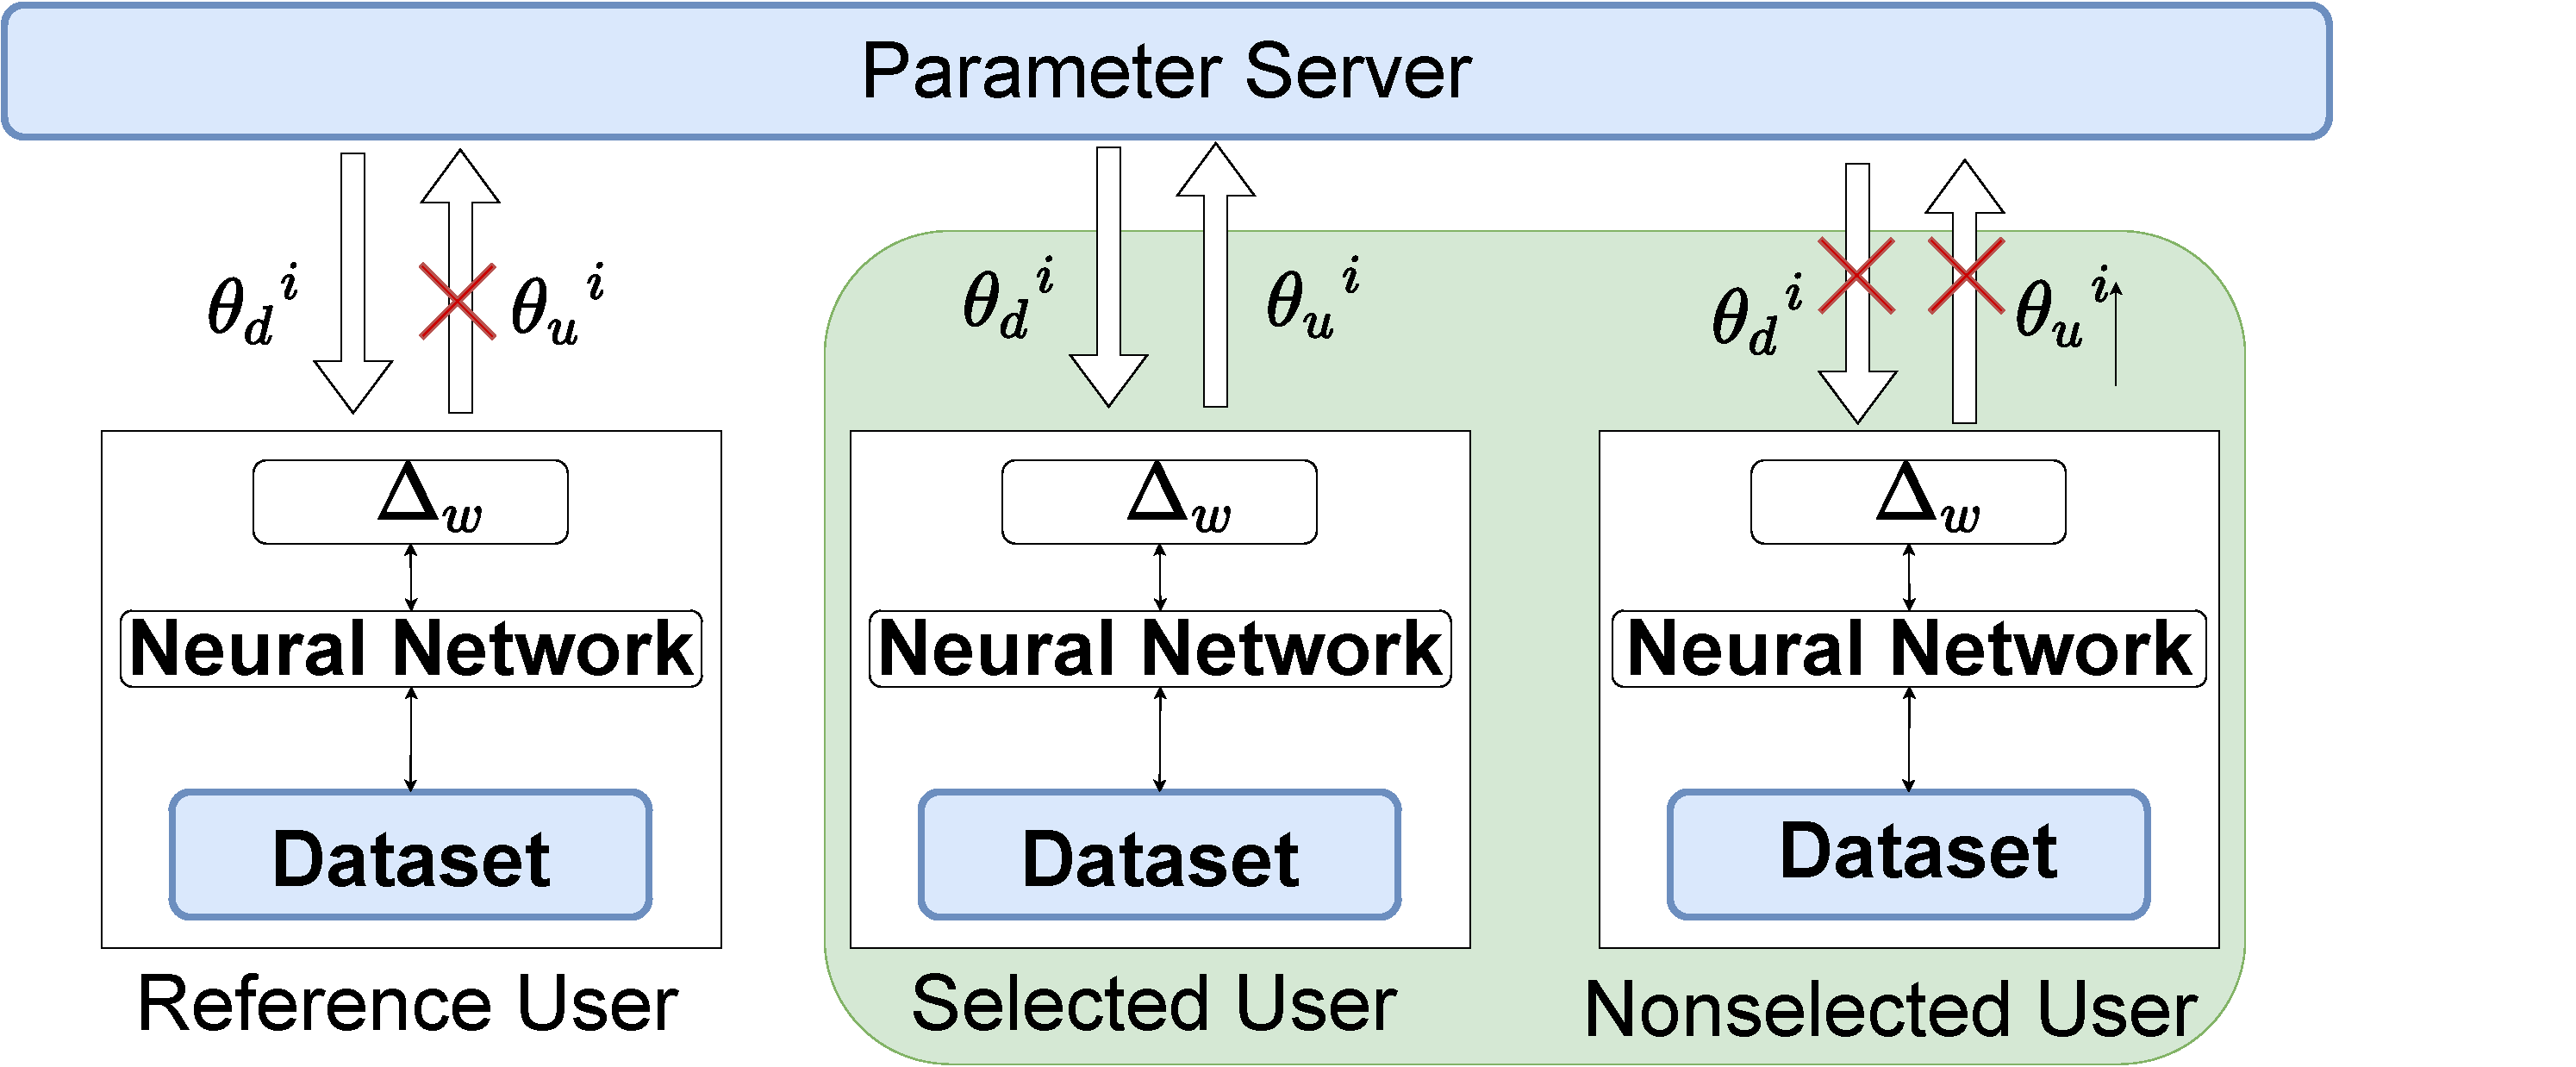
\includegraphics[width=0.5\textwidth, keepaspectratio]{OurHighLevelApproach.pdf}
\caption{One iteration of our proposed algorithm for privacy-preserving distributed learning.}
\label{fig:HighLevel}
\end{figure}
In this section we describe our proposed privacy-preserving distributed learning algorithm that prevents the malicious user from recreating
private samples from other users as described in Section \ref{sec:threatModel}. 
Our main idea is to focus on protecting the privacy of a single users instead of attempting to protect the privacy of all users as in 
\cite{shokri2015privacy}. Our main approach to protect the reference user's privacy is to prohibit the reference user
from uploading its parameters to the  parameter server and only allow the other users to upload their parameters a limited number of
times at randomly chosen iterations.

%Although we focus on the privacy of the reference user, our approach also
%limits the amount of private data that other users expose to an attack. 
%This randomized choosing of participants reduces the chances of selecting the malicious participant in every round, limiting
%the adversary's ability to upload malicious parameters that can force other users to reveal private data. 
%This is in contrast to \cite{shokri2015privacy} where all users participate during all iterations. 

Our proposed algorithm works as follows. 
We assume a reference user $u_0$ aims to train a local deep neural network using its local training data set as well as the
training data sets from other users as described in Section \ref{sec:systemModel}.  We then form a set $\hat{\mathcal{{U}}}$ of
users who upload parameters by randomly selecting each user from the set $\mathcal{U}$ with probability $p$. 
The reference user is never chosen.

User $u_i\in\hat{\mathcal{U}}$ downloads a fraction $\theta_d^i$ of the parameters
in the server, and uses them to overwrite the  corresponding local parameters in $w_i$.
User $u_i$ then trains its network privately using its local data set  $d_i$, and obtains the new parameters $w_i^{(new)}$.
Then, as described in \eqref{eq:deltaParam}, user $u_i$ calculates the change in parameter values by computing $\Delta w_i$, groups the
indexes of the elements in vector $\Delta w_i$ with the largest $\theta_u^i\times |\Delta w_i|$ values in set $\mathcal{S}_i$, and 
forms a vector $w_{\mathcal{S}_i}$ with the elements in $w_i^{(new)}$ that correspond to indexes in $\mathcal{S}_i$. 
User $u_i$ uploads $w_{\mathcal{S}_i}$ to the parameter server who aggregates them. 


After all selected users in $\hat{\mathcal{U}}$ have uploaded their parameters, reference user $u_0$ downloads a fraction $\theta_d^i$
of the aggregated parameters at the server. It then uses the downloaded parameters as initial parameters to retrain its local model.
The iteration
continues until the model at the reference user achieves a minimum accuracy, or until a maximum number of iteration is reached. 

We note that in this algorithm  the reference user  $u_0$ never uploads its parameters to the server, and thus its  private data is
protected from the parameter server and from  malicious users who may attempt to launch the attack in \cite{hitaj2017deep}. 


We summarize our proposed algorithm as follows:

\begin{algorithm}
\begin{algorithmic}[1]
\REQUIRE $\mathcal{U}$
\FOR{$N$ iterations.}
\STATE Choose user $u_i\in\mathcal{U}\setminus u_0$ with probability $p$  and add it to $\hat{\mathcal{{U}}}$.
\FOR{Every $u_i\in\mathcal{U}$}
\STATE User $u_i$ downloads the $\theta_d^i$ of parameters from the server, and replaces the corresponding parameters in $w_i$. 
\STATE User $u_i$ retrains its model using its local data set $d_i$ and obtains the new parameters $w_i^{new}$. 
\STATE User $u_i$ uploads the vector of parameters with the largest change $u_i$ uploads $w_{\mathcal{S}_i}$ to the server.
\ENDFOR
\STATE Reference user $u_0$ downloads all the parameters from the server. 
\STATE Reference user $u_0$ retrains its model using the downloaded parameters and its local data set $d_0$
\IF{Accuracy of model at $u_0$ is equal or grater than $A$.}
\STATE Stop the iteration. 
\ENDIF
\ENDFOR
\ENSURE The parameters $w_0$ at user $u_0$.
\end{algorithmic}
\caption{Our proposed privacy-preserving distributed learning algorithm.}
\end{algorithm}

%-------------------------------------------------------------------------------
\section{Experiment Results}
%-------------------------------------------------------------------------------

To evaluate the performance of our proposed privacy-preserving approach, we implement it on a commercial cloud service provider, and
measure the learning performance of the user $u_0$, and compare it to the learning performance of a centralized deep neural network
architecture that does not protect privacy, and to the distributed learning architecture proposed by Shokri et al. 
\cite{shokri2015privacy} that is vulnerable to the attack in \cite{hitaj2017deep}.

%----------------------------------------------------------------------------
\subsection{Experiment Setup}
%------------------------------------------------------------------------------
We implement all algorithms using Torch with the neural network packages in the scripting language LUAJIT, and run them on an M4
instance on the Amazon Web Service's Elastic Compute Cloud (AWS EC2), which has
2.4 GHz Intel Xeon E5-2676 v3** Processor, 4 VCPUS and 16 GB RAM.
%\begin{figure*}[t]
%\centering
%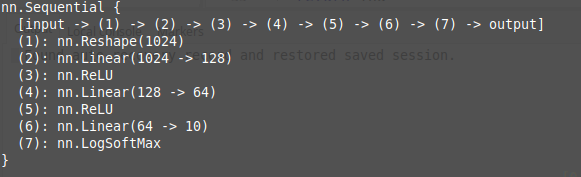
\includegraphics[width = 2 \columnwidth, keepaspectratio]{MLPArchitecture}
%\caption{MLP architecture displaying the tensor size at various stages in the neural network. }
%\label{fig:MLPArch}
%\end{figure*}
As described in Section \ref{sec:systemModel}, we use a 
a multilayer perceptron (MLP) in a feed forward arrangement. The MLP classifies $32\times 32$ pixel images of hand-written numbers. 
Accordingly, our MLP has 1024 input nodes corresponding to each
pixel in the images, and the output layer is a tensor of size 10 where each output corresponds to the probability
that a given input is a specific number
between 0 and 9.  The model has 2 hidden layers where the non-linear ReLU activation function is applied to the
output of each hidden layer.  The first hidden applies a linear transformation
and produces a tensor of size 128 as its output. The second hidden layer accepts a tensor of size 128 as input, and outputs a tensor of
size 64. The last layer of the model is a log soft max layer. 

We trained the MLP using using the MNIST dataset of images of hand-written  numbers\cite{deng2012mnist}. 
The MINST dataset contains 60,000 images in its training dataset and 10,000 images in its test dataset.
%For our experiments, we center the images through a normalization operation.  
To implement our proposed algorithm, we set the size of the local dataset of each participant to 1 \% of the training dataset
images. The reference user starts with a training set of 60 images.
We set the learning rate $\alpha_i$ for all users to $0.1$.  The mini-batch size for stochastic gradient
descent training is set to 10 samples.

%-------------------------------------------------------------------------------
\section{Results}
%-------------------------------------------------------------------------------

% \begin{figure}[!h]
% \centering
% 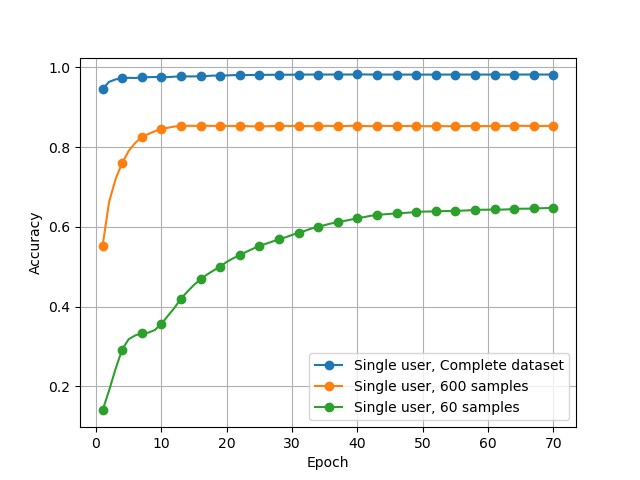
\includegraphics[width=0.8\columnwidth, keepaspectratio]{SingleUserBaselinesGrid}
% \caption{Accuracy under a single user. }
% \label{fig:SingleUser}
% \end{figure}
% To fairly assess the performance improvements offered by our proposed privacy-preserving algorithm, we first measure the accuracy of
% the centralized approach, i.e., a single entity who collects the data from all users but does not provide privacy. 
% Figure \ref{fig:SingleUser} shows the accuracy of the centralized approach for a varying number of epochs. As expected, we see that
% that the accuracy obtained by the centralized approach increases with the number of epochs. 
% 
% Moreover, to assess the performance of users who only have access to their local data set and do not participate in distributed
% learning, we measure the accuracy for different sizes of the local training data set. We see that the accuracy decreases with the
% number of samples in the data set. This confirms that a small local data set without collaboration can only provide a low accuracy to
% the reference user $u_0$.
%We also observe that the accuracy can increase when we use a larger proportion of the data set during training. 
%on a larger
%dataset has a higher accuracy. The user with the highest accuracy has had access to the complete MNIST training dataset of 60,000 samples. 




% We also tested with a scenario in which all participants simply uploaded their local parameters to the server without downloading any
% parameters. Only the reference user was able to download the parameters from the server. In this case, $\theta_d^i$ was 0 for every
% participant except the reference user. 
% \begin{figure}[!h]
% \centering
% 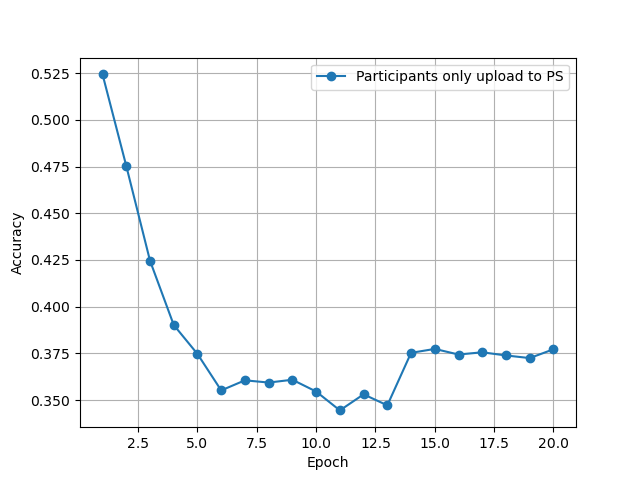
\includegraphics[width=0.8\columnwidth, keepaspectratio]{AllUploadNoDownloadGrid}
% \caption{Accuracy of reference user when all participants simply upload parameters to server. }
% \label{fig:AllUploadNoDownloadGrid}
% \end{figure}


%This approach did not show great results. Figure \ref{fig:AllUploadNoDownloadGrid} shows the accuracy of the reference user is
%negatively impacted in this scenario with each epoch. This shows that downloading the parameters from the server and performing local
%training is a crucial aspect for the efficacy of this architecture.

\begin{figure}[!h]
\centering
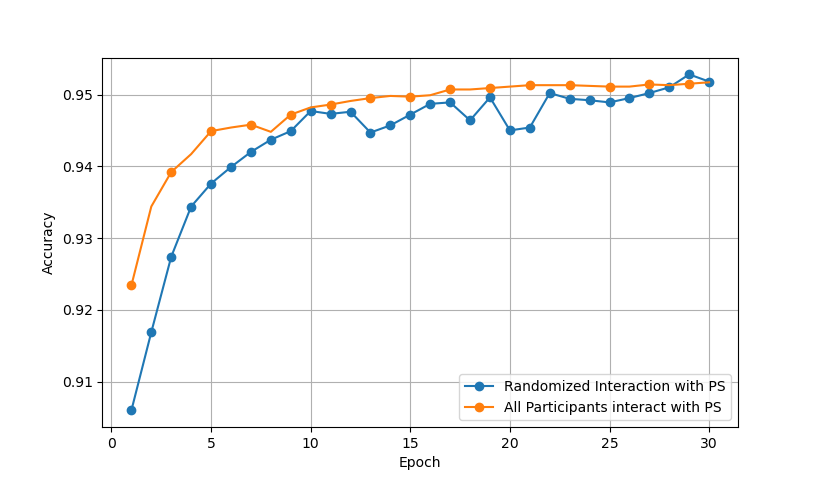
\includegraphics[width=0.9\columnwidth, keepaspectratio]{RandomVsAllGrid}
\caption{Comparison between randomized interaction and complete interaction with server. }
\label{fig:RandVsAll}
\end{figure}
We first compare the accuracy of the reference user under our proposed privacy-preserving algorithm to that of the algorithm proposed
by Shokri et al. \cite{shokri2015privacy}. 
Figure \ref{fig:RandVsAll} shows the accuracy of the reference user $u_0$'s deep learning
neural network trained under our proposed algorithm, and under the algorithm in \cite{shokri2015privacy}. To make a fair comparison, 
we  set the number of users to 20 for both approaches. We set the probability of choosing a non-reference user from $\mathcal{U}$ to
0.5.  In the approach by \cite{shokri2015privacy}, all users upload and download with a probability of 1. 
We see that the reference user $u_0$ is able to obtain a deep learning model with an accuracy that is comparable to the one
obtained by \cite{shokri2015privacy}, which is vulnerable to the attack in \cite{hitaj2017deep}.

\begin{figure}[!h]
\centering
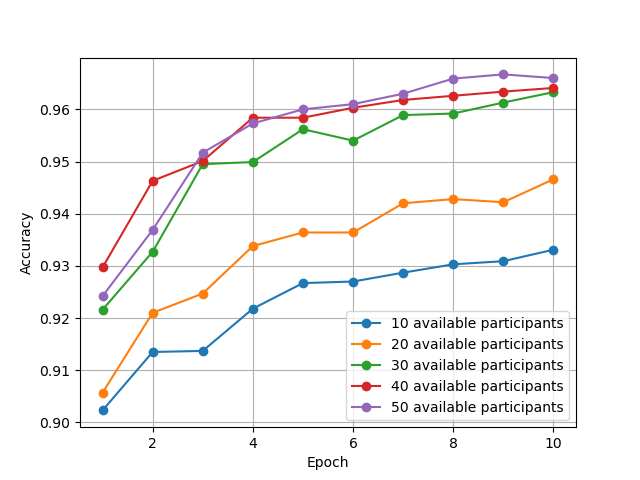
\includegraphics[width=0.9\columnwidth, keepaspectratio]{VaryingPoolofParticipantsGrid}
\caption{Accuracy of Distributed SGD for varying participants available for interaction with the PS.}
\label{fig:VaryingPoolofParticipants}
\end{figure}

We next investigate the impact of the number of non-reference users on the accuracy of the reference user. Figure 
\ref{fig:VaryingPoolofParticipants} shows the accuracy of the reference users $u_0$'s deep neural network under a varying number
of epochs for different numbers of total users in the system. We observe that  the reference user $u_0$ achieves a higher accuracy as
the total number of participants in the system increases. For example, the highest accuracy is achieved with 50 participants, while the
lowest one is achieved with 10 participants. This means the parameters uploaded to the server increases with the number of users, improving 
the accuracy of the model. The reason is that a larger  number of participants brings information from additional local datasets. 

\begin{figure}[!h]
\centering
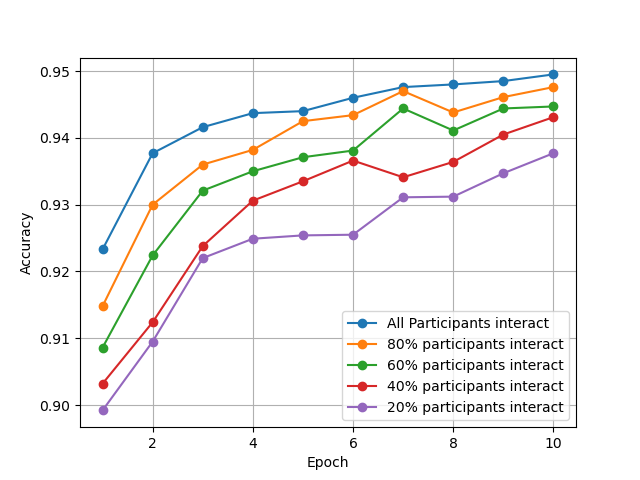
\includegraphics[width=0.9\columnwidth, keepaspectratio]{VaryingProbabilityInteractionGrid}
\caption{Accuracy of Distributed SGD for varying probability of interaction with the PS. }
\label{fig:VaryingProbabilityInteraction}
\end{figure}

Figure \ref{fig:VaryingProbabilityInteraction} shows the accuracy of reference user $u_0$ for different probabilities of choosing
non-reference users $p$ and adding it to $\bar{\mathcal{U}}$.
We see that a greater probability $p$ results in a higher model accuracy for the reference user $u_0$.
The highest accuracy is obtained when all non-reference users are added to the set $\bar{\mathcal{U}}$. 

\begin{figure}[!h]
\centering
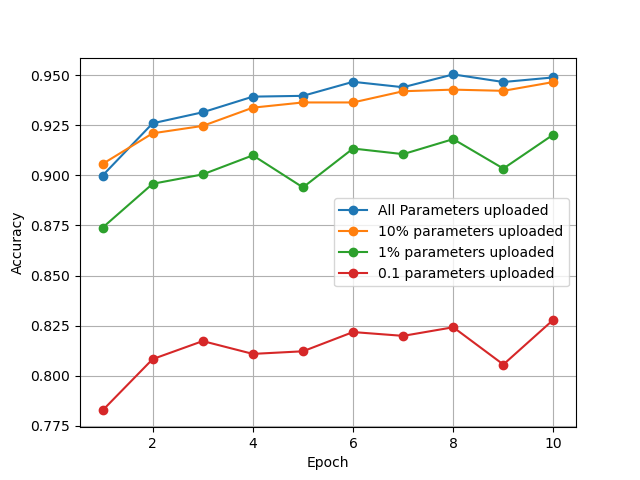
\includegraphics[width=0.9\columnwidth, keepaspectratio]{VaryingThetaUGrid}
\caption{Accuracy of Distributed SGD for different upload gradient selection rate. }
\label{fig:VaryingThetaU}
\end{figure}

In Figure \ref{fig:VaryingThetaU}, we plot the accuracy of the reference user $u_0$ for different upload gradient selection fractions
for the non-reference users. 
The plot shows that the accuracy of $u_0$'s model increases with the percentage of uploaded parameters $\theta_u^i$ (for all $i$) is
However, once value of $\theta_u^i$ reaches 10\% the increase in accuracy for user $u_0$ is small. Thus, by sharing only one tenth
of their parameters, the non-reference users can help $u_0$ achieve a  high accuracy. 



%-------------------------------------------------------------
\section{Conclusion}
%------------------------------------------------------------

In this work, we have investigated the problem of protecting the privacy of a user in distributed training of deep learning models. We
consider a system where a reference user aims to train a model with the help of other users. However, they are unable to directly
share their data sets due to privacy concerns. Although there are some existing works on privacy-preserving distributed training,
they can only protect against semi-honest attacker,i.e., attackers that follow the algorithms,  and are vulnerable to malicious users
that inject specially crafted parameters into the system to compromise the training procedure. To this end, we propose a
distributed training algorithm that protects the privacy of the reference user under these types of attacks. The algorithm only allows
the non-reference users to upload parameters to the server, and thus the reference user's private information is protected. Moreover,
the non-reference users are only allowed to upload parameters at randomly chosen iterations, and thus have a limited ability to
manipulate the training results. Compared to previous works, our solution does not rely on computationally expensive cryptographic
process and can be used with any underlying neural network structure. Our experiment results show that the proposed algorithm can
achieve the same accuracy compared to previous works that are vulnerable to attacks. 

\bibliographystyle{IEEEtran}
\bibliography{references}


\end{document}